\section{Architecture - Modélisation \textsc{SystemC}}

Cette section décrit la modélisation du système en SystemC.

\subsection{Génération du traffic}

Les paquets se présentent sous la forme suivante:
\begin{itemize}
  \item 32 bits (\texttt{int data}) de donnée.
  \item 8 bits (\texttt{uint8\_t address}) d'adresse.
  \item Un champ libre (\texttt{mutable void* extra}) qui permet de rajouter de
    données de contexte suivant ce que l'on veut faire (tracing, statistics,
    \ldots). Celui-ci est rempli à différents endroits stratégiques
    (générateur de trafic, routeur) par des callbacks fournis aux instances
    concernées.
\end{itemize}

\vspace{0.5cm}

Les générateurs de trafic implémentés héritent tous d'une base commune \\
\texttt{noc::abstract\_traffic\_generator} qui leur permet :
\begin{itemize}
  \item D'émettre un paquet aléatoire : \texttt{void
    emit\_random\_package(void)}. Cette fonction remplit le champ \texttt{data}
    par une donnée aléatoire. En revanche entre deux appels, le champ
    \texttt{addresse} fournit reste la même pendant une certaine durée, qui elle
    est aléatoire. Ceci permet de simuler un trafic réaliste. \\
    Une fois le paquet créé, celui-ci est mis à disposition sur le champ
    \texttt{sc\_core::sc\_out<packet> output} et le champ
    \texttt{sc\_core::sc\_out<bool> activated} passe à \texttt{true}. Le champ
    \texttt{activated} reste à \texttt{true} et la fonction est bloquée tant que le champ
    \texttt{sc\_core::sc\_in<bool> acknoledge} n'est pas aquitté par le
    destinataire, ce qui permet d'être sûr de ne perdre aucun paquet sur la
    route. \\
    \textbf{Il faut donc toujours garder en tête que le générateur de traffic
      n'ira pas toujours à la vitesse demandée mais sera borné par la capacité
      à absorber les paquets du destinataire. Attention donc aux interprétations
      de résultat hâtives.}
  \item De pourvoir le module d'un callback de type
    \texttt{std::function<void(noc::packet)>} qui sera appelé à la création de
    chaque paquet.
\end{itemize}

\subsubsection{Les générateurs fournis}

\paragraph{\texttt{stream\_generator} \\}

Ce générateur de traffic émet des paquets à une fréquence fixe. On utilisera sa
methode \texttt{void set\_period(unsigned period)} pour régler cette fréquence.

\paragraph{\texttt{burst\_generator} \\}

Ce générateur possède trois paramètres:
\begin{itemize}
  \item La fréquence des bursts.
  \item La fréquence d'émission des paquets lors d'un burst.
  \item La quantité de paquet émits lors d'un burst.
\end{itemize}
On utilisera la methode \texttt{void set\_burst(unsigned long\_period, unsigned
short\_period, unsigned burst\_length)} pour fixer ces valeurs.

\subsection{Routeur}

Nous faisons correspondre à chaque entrée du système un module routeur, connecté
à autant de FIFO qu'il y a de sorties au système.

Chacun de ces modules reçoit alors les données correspondant à son entrée en
suivant un mécanisme de synchronisation de type handshake.

Sur un front montant de l'horloge, si le signal d'activation a une valeur positive,
le routeur lit un paquet et détermine la FIFO dans laquelle celui-ci doit être placé.
Le routeur lit ensuite le nombre d'emplacements libres de cette FIFO.
Si ce nombre est non nul, le paquet peut être écrit dans la FIFO.
Sinon, le routeur attend que la FIFO se désemplisse.
Une fois le paquet écrit dans la FIFO, le routeur émet un signal d'acquittement,
puis attend que le signal d'activation reprenne une valeur négative.
Une nouvelle valeur pourra alors être reçue suivant le même protocole.

\subsection{Arbitrage}

Similairement, nous faisons correspondre à chaque sortie du système un module
d'arbitrage, connecté à autant de FIFO qu'il y a d'entrées au système.
Chacun de ces modules reçoit également en entrée un signal définissant un choix
de stratégie d'arbitrage, déterminant dans quel ordre
les paquets en provenance des différentes entrées doivent être écrites en
sortie.

Dans la mesure où le choix de stratégie d'arbitrage peut changer à tout moment,
l'arbitrage se fait en 5 temps:
\begin{enumerate}
  \item lecture du choix de stratégie d'arbitrage
  \item détermination de la FIFO sur laquelle lire le paquet (suivant la stratégie
    d'arbitrage choisie)
  \item lecture du paquet dans la FIFO correspondante (s'il y a au moins une FIFO
    non vide)
  \item écriture du paquet en sortie (ou d'une valeur par défaut si toutes les
    FIFO sont vides)
  \item et mise à jour de l'état interne du module en vue d'arbitrages futurs
\end{enumerate}
La suite de cette partie détaille les différentes stratégies d'arbitrage
 modélisées et leur mise en œuvre.

\subsubsection{Arbitrage suivant des priorités fixes}

Il s'agit de la stratégie d'arbitrage la plus simple: choisir la FIFO non vide
la plus prioritaire.

Pour chaque FIFO, en suivant un ordre déterminé, le module lit donc le signal
correspondant au nombre de paquets disponibles. La première FIFO non vide est
alors choisie.

\subsubsection{Arbitrage en tourniquet}

Il s'agit d'une stratégie assez similaires à la précédente. Le module choisit
ici aussi la première FIFO non vide, en parcourant celles-ci dans un ordre
déterminé, mais cette fois il les parcourt à partir de la dernière FIFO lue.

Cette stratégie d'arbitrage nécessite de savoir à tout instant quelle est la
dernière FIFO à avoir été lue. Il faut donc stocker cette information et la
mettre à jour après chaque lecture.

\subsubsection{Arbitrage par choix de la moins récente utilisation}

Il s'agit cette fois de choisir la FIFO la moins récemment choisie.

La mise en œuvre de cette stratégie repose sur l'utilisation d'un registre
interne dans lequel on stocke les indices des FIFOS par date de dernière
utilisation, de la moins récente à la plus récente. Le module  choisit alors la
première FIFO non vide, en parcourant celles-ci dans l'ordre où leurs indices
sont stockés dans le registre.

Après une lecture, pour mettre à jour le registre, on décale vers le début de
celui-ci toutes les valeurs situées après celle correspondant à l'indice de la
FIFO lue. Cette dernière est ensuite écrite dans la dernière case du registre.

\subsubsection{Arbitrage de type FIFO}

Cette stratégie d'arbitrage est la plus complexe de celles présentées ici: les
paquets doivent être lus dans leur ordre d'arrivée, quelle que soit la FIFO dans
laquelle ils ont été placés.

Pour arriver à ce résultat, le module utilise un registre interne, initialement
vide. A chaque fois qu'une variable est écrite dans une des FIFOs, l'indice de
cette FIFO est écrit dans ce registre à une position correspondant au nombre de
paquets présents dans l'ensemble des FIFOs. Inversement, à chaque fois qu'un
paquet est lu dans une FIFO, la première occurrence de l'indice de cette variable
dans le registre est supprimée. Les valeurs du registres situées après cette
occurrence sont ensuite décalées vers le début du registre.

Ainsi, la première case du registre correspond toujours à l'indice de la FIFO
contenant le paquet le plus ancien.

\subsubsection{Arbitrage aléatoire}

Pour choisir aléatoirement une FIFO dans laquelle lire, le module génère des
nombres aléatoires à l'aide d'un registre à décalage à rétroaction linéaire. Ce
nombre est ensuite ramené entre 0 et le nombre de FIFOs non vides, ce qui
indique laquelle d'entre elles doit être choisie.


\subsection{Résultats}

Nous avons suivi les paquets passant par notre système pour chacun des modes
d'arbitrage et en faisant varier la profondeur des FIFO présentes entre les
routeurs et les arbitreurs ainsi que la fréquence d'emmission du générateur (ici
un \texttt{stream\_generator}). Nous obtenons ainsi tout un tas de statistiques
intéressantes par l'intermédiaire de scripts \textsc{matlab}. \\
Une d'entre elle en particulier nous a permis de définir les objectifs à
atteindre en terme de fréquence d'horloge du système:

\begin{figure}[!h]
  \centering
  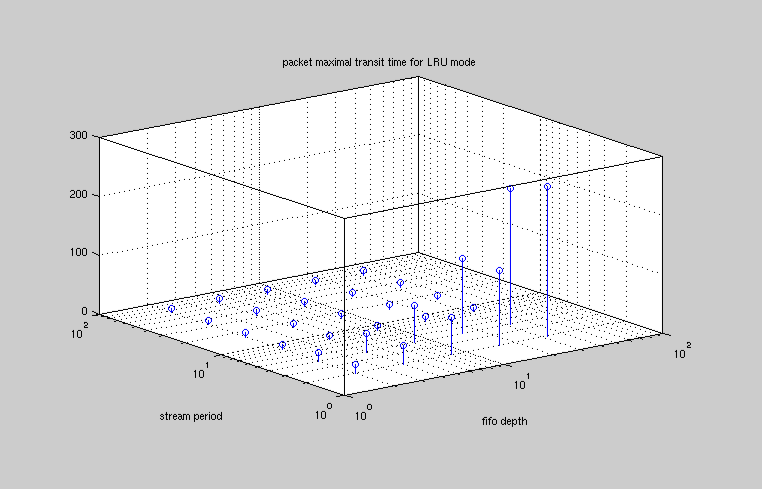
\includegraphics[width=\textwidth]{./data/max_transit_time.png}
  \caption{Durée maximale de transit d'un paquet à travers le switch en
    fonction de la période ($2^i$ coups d'horloge) d'emmission du générateur
    de paquet et de la profondeur de \textsc{fifo} du switch ($2^i$ registres)}
\end{figure}

En effet, on remarque que pour que les FIFO ne soient pas saturées en permanence
et qu'elle ne ralentisse donc pas le flux de données entrant, il faut qu'un
paquet arrive au minimum tous les huit coups d'horloge. Sachant que le débit
imposé est de $100Mbit/s$ pour chaque sortie du NOC, et que nos paquets portent
32 bits de donnée, notre fréquence d'horloge doit être donc supérieure à:
\[
  f_{saturation} = \frac{100\ \mbox{Mbit/s}}{32\ \mbox{bit}}
    \times \frac{32\ \mbox{output}}{4\ \mbox{input}}
    \times 8\ \mbox{clock} =
  200\ \mbox{MHz}
\]

Ensuite la durée de transit maximale est alors de 9 coups d'horloge. Or la
latence maximale imposée est de 80ns. Obtient donc une deuxième contrainte:
\[
  f_{latence} = \frac{9\ \mbox{clock}}{80\ \mbox{ns}} = 112.5\ \mbox{MHz}
\]

